\documentclass[t, 				             
			   final,
			   12pt, 				         
			   xcolor={usenames,dvipsnames}, 
			   table]{beamer}

% pacotes utilizados.
\usepackage[alf]{abntex2cite}
\usepackage{amsmath}
\usepackage[brazil]{babel}
\usepackage{booktabs}
\usepackage{caption}
\usepackage[utf8]{inputenc}
\usepackage{listings}
\usepackage{multicol}
\usepackage{multirow}
\usepackage{todo}


% configuração do tema
\usetheme[pageofpages=de,
          bullet=square,			
          titleline=true,				
          alternativetitlepage=true,			
          titlepagelogo=imagens/logo-puc,	
          watermarkheight=70px,		
          watermarkheightmult=4	
          ]{Torino}

\setbeamertemplate{sections/subsections in toc}[square]
\setbeamertemplate{bibliography item}[default]

\usecolortheme{freewilly}

% Block Environment
% -------------------------------
\setbeamertemplate {blocks}[default]
\setbeamercolor{block title}{fg=red!0!green!15!blue!85!, bg=red!33!green!37!blue!15!}
\setbeamercolor{block body}{fg=black, bg=red!32!green!33!blue!5}
\setbeamercolor{block title alerted}{fg=white, bg=red!40!black}
\setbeamercolor{block body alerted}{fg=black, bg=red!5!white}
\setbeamercolor{block title example}{fg=white, bg=green!40!black}
\setbeamercolor{block body example}{fg=black, bg=green!5!white}
\setbeamerfont{block title}{size=\scriptsize, series=\bfseries}


\definecolor{javared}{rgb}{0.6,0,0} % for strings
\definecolor{javagreen}{rgb}{0.25,0.5,0.35} % comments
\definecolor{javapurple}{rgb}{0.5,0,0.35} % keywords
\definecolor{javadocblue}{rgb}{0.25,0.35,0.75} % javadoc
 
\lstset{}

\lstdefinestyle{BashInputBasicStyle}{
	language=bash,
	basicstyle=\normalsize\ttfamily,
	columns=fullflexible,
	tabsize=2,
	showstringspaces=false,
	frame=single,
	inputencoding=utf8,
	rulecolor=\color{gray}
}

\lstdefinestyle{BashInputStyle}{
  language=bash,
  basicstyle=\normalsize\ttfamily,
  numbers=left,
  numberstyle=\tiny,
  numbersep=2pt,
  frame=tb,
  columns=fullflexible,
  tabsize=2,
  showstringspaces=false,
  commentstyle=\color{gray},
  inputencoding=utf8,
  rulecolor=\color{gray}
}

\lstdefinestyle{RubyInputStyle}{
    language=ruby,
    basicstyle=\scriptsize\ttfamily,
    keywordstyle=\color{javapurple},
    identifierstyle=\color{black},
    commentstyle=\color{javagreen},
	stringstyle=\color{blue},
    showstringspaces=false,
    numbers=left,
    numberstyle=\color{gray}\tiny,
    tabsize=3,
    extendedchars=\true,
    inputencoding=utf8,
%   frame=single, 
    columns=fixed,
    backgroundcolor=\color{red!32!green!33!blue!5}
}    
%  language=ruby,
%  basicstyle=\normalsize\ttfamily,
%  keywordstyle=\color{OrangeRed},
%  identifierstyle=\color{Turquoise},
%  commentstyle=\color{gray},
%  stringstyle=\color{YellowOrange},
%  numbers=left,
%  numberstyle=\tiny,
%  numbersep=2pt,
%  frame=tb,
%  columns=fullflexible,
%  backgroundcolor=\color{white!80},
%  linewidth=0.9\linewidth,
%  tabsize=2,
%  showstringspaces=false
%  inputencoding=utf8


\lstdefinestyle{JavaInputStyle}{
	language=Java,
	basicstyle=\ttfamily,
	keywordstyle=\color{javapurple}\bfseries,
	stringstyle=\color{javared},
	commentstyle=\color{javagreen},
	morecomment=[s][\color{javadocblue}]{/**}{*/},
	numbers=left,
	numberstyle=\tiny\color{black},
	numbersep=10pt,
	tabsize=2,
	showspaces=false,
	showstringspaces=false,
	frame=tb,
	columns=fullflexible,
	backgroundcolor=\color{white!80},
	linewidth=0.9\linewidth,
	inputencoding=utf8
}

\begin{document}
	\author{Luiz Alberto Ferreira Gomes}
\title{Aula 03: Ruby On Rails}
\subtitle{Laboratório de Projeto de Sistemas}
\institute{Curso de Ciência da Computação}
\date{\today}

	\begin{frame}[plain]
  \titlepage
\end{frame}
	\AtBeginSection[]
{
  \begin{frame}{Agenda}
    \tableofcontents[currentsection]
  \end{frame}
}
  	

  	\section{Páginas Estáticas}
		%---------------------------------------------------------------------[ Início ]
\begin{frame}[allowframebreaks, fragile,t]{Controladores e Ações}
    \begin{itemize}
      \item Um controlador Rails pode ser gerado utilizando o comando \alert{rails 
	generate controller} ou \alert{rails g controller}.Além dele, esse comando permite 
	a geração de algumas ações.
    \end{itemize}
      \begin{lstlisting}[style=BashInputStyle]
 ~/blog$ rails generate controller Home index help
 route  get 'home/help'
 route  get 'home/index'
 invoke  erb
 create    app/views/home
 create    app/views/home/index.html.erb
 create    app/views/home/help.html.erb
 ...
      \end{lstlisting}
\end{frame}

%---------------------------------------------------------------------[ Início ]
\begin{frame}[allowframebreaks, fragile,t]{Arquivo de Roteamento: routes.rb}
    \begin{itemize}
      \item O conteúdo atualizado do arquivo \alert{routes.rb} deverá conter as notas rotas 
	para as ações recém-criadas.
	  \begin{lstlisting}[style=RubyInputStyle, caption=config/routes.rb]
	    Rails.application.routes.draw do
	      get 'home/index'
	      get 'home/help'
	      root 'home#index'
	      resources :posts 
	    end 
	  \end{lstlisting}
    
      \item \alert{GET} é uma das operações do HTTP mais comuns, ela é utilizada para a leitura
      de dados na web.
      \begin{itemize}
	\item o navegador envia uma requisição \alert{GET} toda vez de se deseja visitar um endereço, com por exemplo \url{http://www.inf.pucpcaldas.br}. 
       
      \end{itemize}

      \item As páginas vinculadas às ações \alert{index} e \alert{help} podem ser 
	visitadas, primeiro, iniciando o servidor Rails com os comandos \alert{rails server} ou, 
	simplesmente, \alert{rails s}.
	
	\begin{lstlisting}[style=BashInputStyle]
	  $ cd ~/workspace/blog
	  $ rails server
	\end{lstlisting}
    
      \item E depois, digitando as páginas os endereços \alert{\url{http://localhost:3000/home/index}} e, depois, \alert{\url{http://localhost:3000/home/help}}.
      
    \end{itemize}
    
\end{frame}


		
%---------------------------------------------------------------------[ Início ]
\begin{frame}[allowframebreaks, fragile,t]{Página Home}
    \begin{itemize}
      \item  A páginas geradas pelo comando \verb!rails generate! devem ser personalizadas para
	atenderem às especificações do projeto da aplicação. Por exemplo, para a página associada à ação principal
	pode-se reescrevê-la da seguinte forma:
	    \begin{lstlisting}[style=RubyInputStyle, basicstyle=\tiny\ttfamily, caption=app/views/home/index.html.erb]
<!DOCTYPE html>
<html>
   <head>
      <title>Index | Blog App</title>
   </head>
   <body>
      <h1>Blog App</h1>
      <p>
         Esta e a pagina index da aplicacao Blog desenvolvida durante
         o Laboratorio de Engenharia de Software.
      </p>
   </body>
</html>
	    \end{lstlisting}
    
      \item Já para a página associada à ação ajuda pode-se reescrevê-la, por exemplo, da seguinte forma:
	    \begin{lstlisting}[style=RubyInputStyle, basicstyle=\tiny\ttfamily, caption=app/views/home/help.html.erb]
<!DOCTYPE html>
<html>
   <head>
      <title>Help | Blog App</title>
   </head>
   <body>
      <h1>Blog App</h1>
      <p>
         Esta e a pagina help da aplicacao Blog desenvolvida durante
         o Laboratorio de Engenharia de Software.
      </p>
   </body>
</html>
	    \end{lstlisting}
    \end{itemize}
    
\end{frame}
		\section{Estruturando a Aplicação}
%---------------------------------------------------------------------[ Início ]
\begin{frame}[fragile,t]{Criando Um Helper}
    \begin{itemize}
      \item  Um helper será criado para promover o reúso e evitar a repetição 
        de código em uma aplicação. 
    \end{itemize}
      \begin{lstlisting}[style=RubyInputStyle, basicstyle=\tiny\ttfamily, firstline=1, lastline=10, caption=app/helpers/application\_helper.rb]
module ApplicationHelper
    def preenche_titulo(titulo_da_pagina='')
        titulo_padrao="Blog App"
        if (titulo_da_pagina.empty?)
            titulo_padrao
        else
            "#{titulo_da_pagina} | #{titulo_padrao}"
        end
    end
end
      \end{lstlisting}
\end{frame} 
%---------------------------------------------------------------------[ Início ]
\begin{frame}[fragile,t]{Estruturando a Aplicação}
    \begin{itemize}
      \item  Uma aplicação web deve ser estruturada de forma a facilitar o seu uso.
        Uma ferramentas utilizadas para isso é o protótipo essencial. A ideia inicial
        para a aplicação Blog foi pensada. 
      \begin{figure}[h!]
        \centering
        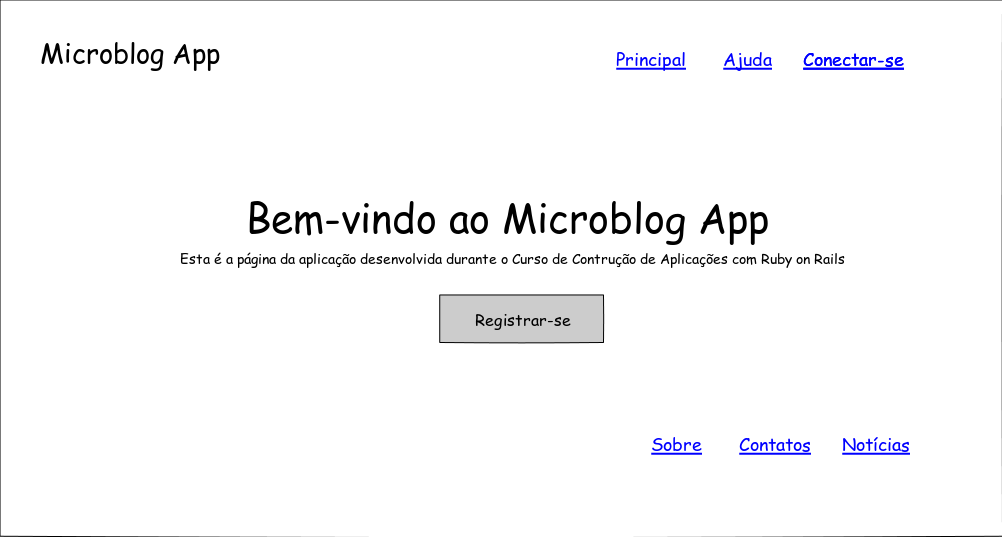
\includegraphics[width=0.65\textwidth]{imagens/esboco-da-pagina-principal.png}
      \end{figure}
    \end{itemize}
\end{frame} 

%---------------------------------------------------------------------[ Início ]
\begin{frame}[allowframebreaks, fragile,t]{Navegação da Aplicação}
      \begin{lstlisting}[style=RubyInputStyle, basicstyle=\tiny\ttfamily, caption=app/views/layouts/application.html.erb]
<!DOCTYPE html>
<html>
<head>
  <title><%= preenche_titulo(yield(:titulo)) %></title>
  <%= stylesheet_link_tag    'application', media: 'all', 
      'data-turbolinks-track' => true %>
  <%= javascript_include_tag 'application', 'data-turbolinks-track' => true %>
  <%= csrf_meta_tags %>
</head>
<body>
  <%= link_to "Blog", "#", id: "logo" %>
  <p>
    <ul>
      <li><%= link_to "Index", home_index_path %></li>
      <li><%= link_to "Help", home_help_path %></li>
    </ul>
  </p>
  <%= yield %>
</body>
</html>
      \end{lstlisting}
\end{frame} 

%---------------------------------------------------------------------[ Início ]
\begin{frame}[allowframebreaks, fragile,t]{Refatorando as Páginas Index e Help}
   \begin{lstlisting}[style=RubyInputStyle, basicstyle=\tiny\ttfamily, caption=app/views/home/index.html.erb]
<%= provide :titulo, "Index" %>
<div>
    <h1>Blog App</h1>
    <p>
      Esta e a pagina principal da aplicacao Blog desenvolvida durante 
      o Laboratorio de Engenharia de Software.
    </p>
    <%= link_to "Posts", posts_path %>
</div>      
  \end{lstlisting}
  
   \begin{lstlisting}[style=RubyInputStyle, basicstyle=\tiny\ttfamily, caption=app/views/home/help.html.erb]
<%= provide :titulo, "Help" %>
<div>
    <h1>Blog App</h1>
    <p>
      Esta e a pagina de ajuda da aplicacao Blog desenvolvida durante 
      o Laboratorio de Engenharia de Software.
    </p>
</div>      
  \end{lstlisting}
\end{frame} 

  	\section{Para Saber Mais}
		%%-------------------------------------------------------------------------------------- Início
\begin{frame}[fragile,t]{Para Saber Mais}
  \begin{itemize}
    \item \url{https://www.ruby-lang.org/en/}
    \begin{itemize}
     \item referência oficial da linguagem Ruby onde a toda a sua documentação está disponível
	para ser consultada.
    \end{itemize}

    \item \url{http://rubyonrails.org/}
    \begin{itemize}
     \item referência oficial do framework Rails onde a toda a sua documentação está disponível
	para ser consultada.
    \end{itemize}
    
    \item \url{http://www.codecademy.com/pt/tracks/ruby}
    \begin{itemize}
     \item curso iterativo em portugês sobre a linguagem Ruby.
    \end{itemize}

	\item \url{https://gorails.com/setup/ubuntu/16.04}
	\begin{itemize}
		\item guia para instalação do Ruby on Rails no Ubuntu e no Mac OSX.
	\end{itemize}
  \end{itemize}
  
  
\end{frame}
\end{document}
